\section{Contrôle}
Pour des raisons de simplicité, le programme est entièrement contrôlable à la souris, en interaction directe sur la représentation du cube serpent et la caméra et indirecte par les menus et les boutons suivant-précédent.
La caméra est de type "vue à la troisième personne libre": le clic droit permet de la déplacer sur une sphère centrée sur un point, le clic du milieu permet de déplacer ce point central sur le plan (xz) et la molette permet de modifier le rayon de cette sphère.
On interagit avec le casse-tête grâce au clic gauche, qui permet de sélectionner/désélectionner un cube et de le faire tourner, faisant ainsi tourner le reste du serpent dans sa course.
Il existe aussi quelques raccourcis clavier permettant d'avoir un contrôle plus rapide sur le programme: <entrée> permet de visualiser les liens entre cubes, "droite" et "gauche" servent de suivant-précédent et "haut" sert à remettre le casse-tête à plat.
Le menu et les boutons suivant-précédent seront détaillés par la suite.

\section{Sélection}

Sélectionner un cube n'est pas une tâche simple du côté du code: en effet, il ne nous est pas possible avec les données dont nous disposons de savoir simplement quel cube est sous la souris au moment d'un clic. Il existe cependant quelques techniques apportant des solutions à se problème, comme la création de "hit-boxes", la transformation inverse de caméra et le color-picking. La plus adéquate dans notre cas est la dernière, pour des raisons de précision et de simplicité.

Le color picking consiste à rendre une image ayant la même géométrie que le rendu classique, mais où chaque couleur de pixel correspond à une information: chaque cube est rendu avec une couleur permettant de l'identifier. Dans notre cas, nous avons décidé de coder l'identifiant du cube sur le canal rouge : 0 signifiant le premier cube et 255 aucun.

Les menus sont codés sur le canal vert : 0 signifiant le premier item et 255 aucun.

Les cubes apparaissent donc en nuances de vert, leur couleur étant codée de cette manière : rouge=255, vert=identifiant, bleu=0 et les menus apparaissent en nuance de rouge, étant codés comme suit: rouge = identifiant, vert=255, bleu=0.

L'image est rendue dans une texture (et non à l'écran !), on peut alors lire le pixel que pointe la souris pour savoir quel élément de l'image l'utilisateur à sélectionné.

\begin{figure}[h]
 \centering
 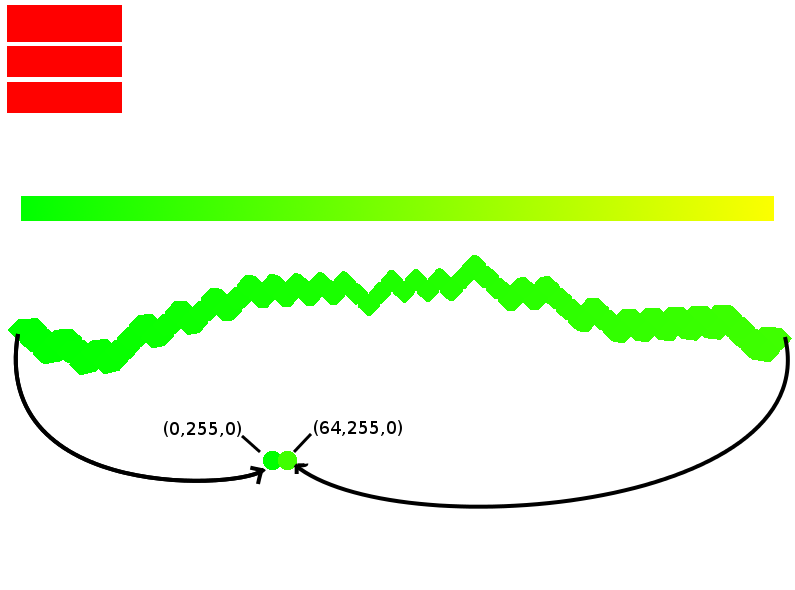
\includegraphics[scale=0.3,keepaspectratio=true]{img/colorpick.png}
 \caption{Rendu du color-picking}
 \label{colorPick}
\end{figure}

\section{Menu}
Dans l'optique de fournir un contrôle de l'application exclusivement à la souris, nous avons donc crée deux interfaces pour l'application.
Un jeu de deux boutons de part et d'autres de la représentation 2D du serpent à plat qui déclenche des actions différentes selon le mode de jeu.\newline

En mode jeu le bouton droit permet de demander de l'aide à l'application pour qu'elle calcule la prochaine étape de solution. Le gauche quant à lui permet d'annuler notre action et donc de revenir a l'état précédant du casse-tête en résolution.\newline

En mode solution les boutons droite et gauche servent respectivement à parcourir la résolution d'avant en arrière pour pouvoir résoudre le casse tête physique.\newline

L'autre interface est un menu dynamique permettant diverse actions sur l'application tel que le chargement d'un autre template de serpent, parcourir les solutions, quitter le programme (nous vous laisserons découvrir tout ceci dans le guide d'utilisation !).
